 \begin{figure}
	\begin{center}
	%	\def\svgwidth{1.0\textwidth}
	%	\input{pics_tex/caustica1.pdf_tex}
	 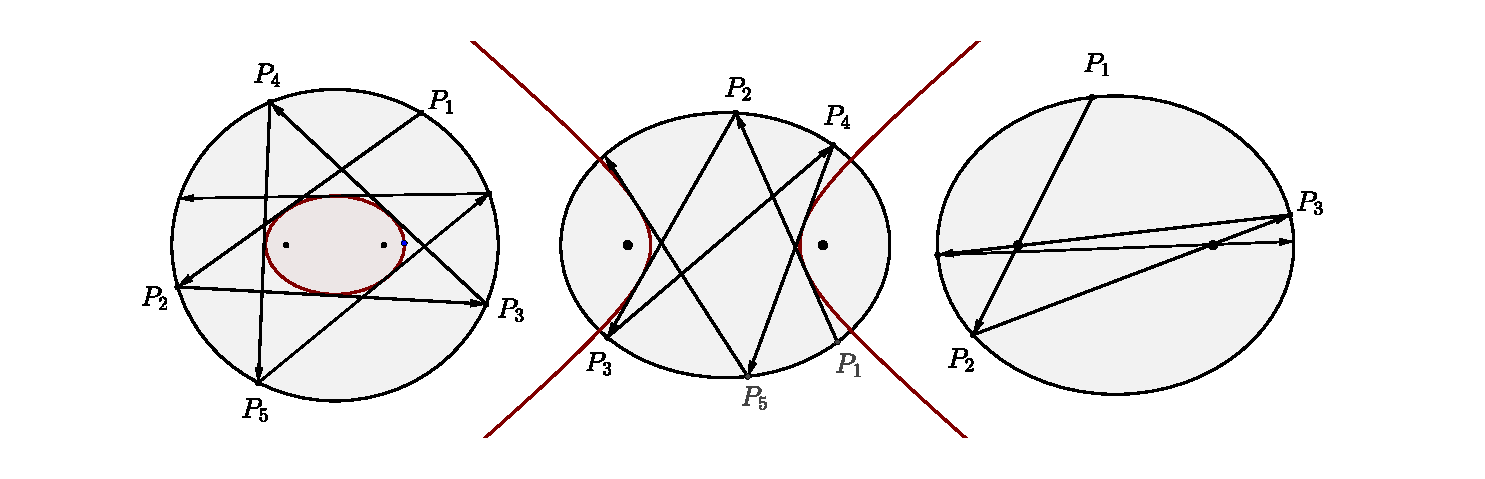
\includegraphics[scale=0.55]{chap_05/pics/pics-05-3tipos-orbitas.pdf}
		\caption{Three types of billiard orbits in the ellipse.}
	\end{center}
\label{fig:caustic1}
\end{figure} 
 
 \begin{theorem}
 Consider an  elliptic billiard defined  in the ellipse $\E$ given by $x^2/a^2+y^2/b^2=1$ $(a>b)$. Let $F_1=(-c,0)$ and $F_2=(c,0) $ the foci of $\E$. Let $(P_n)=(P_n)_{n\in\mathbb{Z}}$ be a billiard orbit inscribed in $\E$. Then:
 
 \begin{itemize} 
 \item[i)] If the segment of orbit $P_1 P_2$ is outside the segment $F_1F_2$ then the caustic of the orbit $(P_n)$ is a confocal ellipse $\E_c$ and the orbit is periodic or dense in the annulus defined by the pair  $\{\E,   \E_c \}$.
 
  \item[ii)] If the segment of orbit $P_1P_2$   intersects the segment $F_1F_2$ then the caustic of the orbit is a confocal hyperbola  $\Hc_1$ and the orbit is periodic or dense in the disk defined by the ellipse $\E$ and the caustic $\Hc_1$.
  
   \item[iii)] If the segment of orbit $P_1P_2$ pass through a focus  then the orbit pass through the other focus and is asymptotic to the 2-periodic orbit (diameter of the ellipse $\E$) in the past (backward) and  the future(forward).
\end{itemize}
\end{theorem}

 \begin{proof}
 We follow \cite{bry-2010} to obtain the billiard map as a composition of two deck transformations.  Consider the pair of nested   ellipses parametrized by
 
 \begin{align*}
     \E:&\;\; f(z,w)=\frac{z^2}{a^2}+\frac{w^2}{b^2}-1=0\\
     \E_c:&\;\; g(x,y)= \frac{x^2}{a_c^2}+\frac{y^2}{b_c^2}-1=0.
 \end{align*}
 
 A tangent (oriented) line to $\E_c$ (caustic), passing through $q_0=(x,y)$ is given by
 \[h(x,y,z,w) =\frac{xz}{a_c^2}+\frac{yw}{b_c^2}-1=0.\]
 Now consider the set
 $\Sigma= \{(x,y,z,w): f(z,w)=g(x,y)=h(x,y,z,w)=0\}.$  
 The set $\Sigma$ is the union of two disjoint circles (curves  diffeomorphic  to circles) given by
 $\Sigma_+=\{p\in \Sigma: xw-yz>0\} $ and
  $\Sigma_-=\{p\in \Sigma: xw-yz<0\}. $
  Given $q_0\in\E_c$, let $p_0=(z,w)\in \E$ such that $(q_0,p_0)\in\Sigma_+.$ A line passing through $p_0$ and tangent to $\E_c$ passes through the point $q_1=(u,v)$ and $(u,v,z,w)\in\Sigma_-.$ 
 The projection  $\pi_1:\Sigma \to \E_c$ is a double cover. The same for the projection
 and $\pi:\Sigma\to \E$. 
 Now we observe that there is a unique map $\tau:\Sigma_{\pm}\to \Sigma_{\mp}$ such that $\tau(x,y,z,w)=(x,y,\bar{z},\bar{w})$. Here $(\bar{z},\bar{w})$ is the other point of intersection of the tangent line passing $(x,y)$ with the outer ellipse $\E$.
 
Also there is a unique map $\sigma:\Sigma_{\pm}\to \Sigma_{\mp}$ such that $\tau(x,y,z,w)=( \bar{x},\bar{y},z,w)$. The point $q_1=( \bar{x},\bar{y})\in\E_c$ is the in polar line of $p_0=(z,w)$. 
 
 %%%
 
 Therefore the billiard orbit can be defined as follows. For each $q_i\in \E_c$, let $p_i\in\E$ the point of intersection of tangent line at $q_i$ to $\E_c$ meets $\E$ with $(q_i,p_i)\in\Sigma_{+}$. Now let $q_{i+1}$ be the unique point on $\E_c$ such that $\{q_i,q_{i+1}\}$ are on the two tangent lines to $\E_c$ that pass through $p_i$. Therefore,   the map $q_i\to q_{i+1}$ is given by $\sigma\circ \tau$ (resp. $p_i\to p_{i+2}$) is an orientation preserving diffeomorphism on $\E_c$ (resp. on $\E$).

When the caustic is a hyperbola it is necessary to consider the second iteration to obtain an orientation diffeomorphism. See \cite{birkhoff1922} and \cite{kolod1985}.

Finally, when the orbit passes through a focus, the billiard map is conjugated with a diffeomorphism of the circle having two hyperbolic fixed points.
\end{proof}
 


\begin{figure}
	\begin{center}
	%	\def\svgwidth{1.0\textwidth}
	%	\input{pics_tex/bilharorbita.pdf_tex}
		 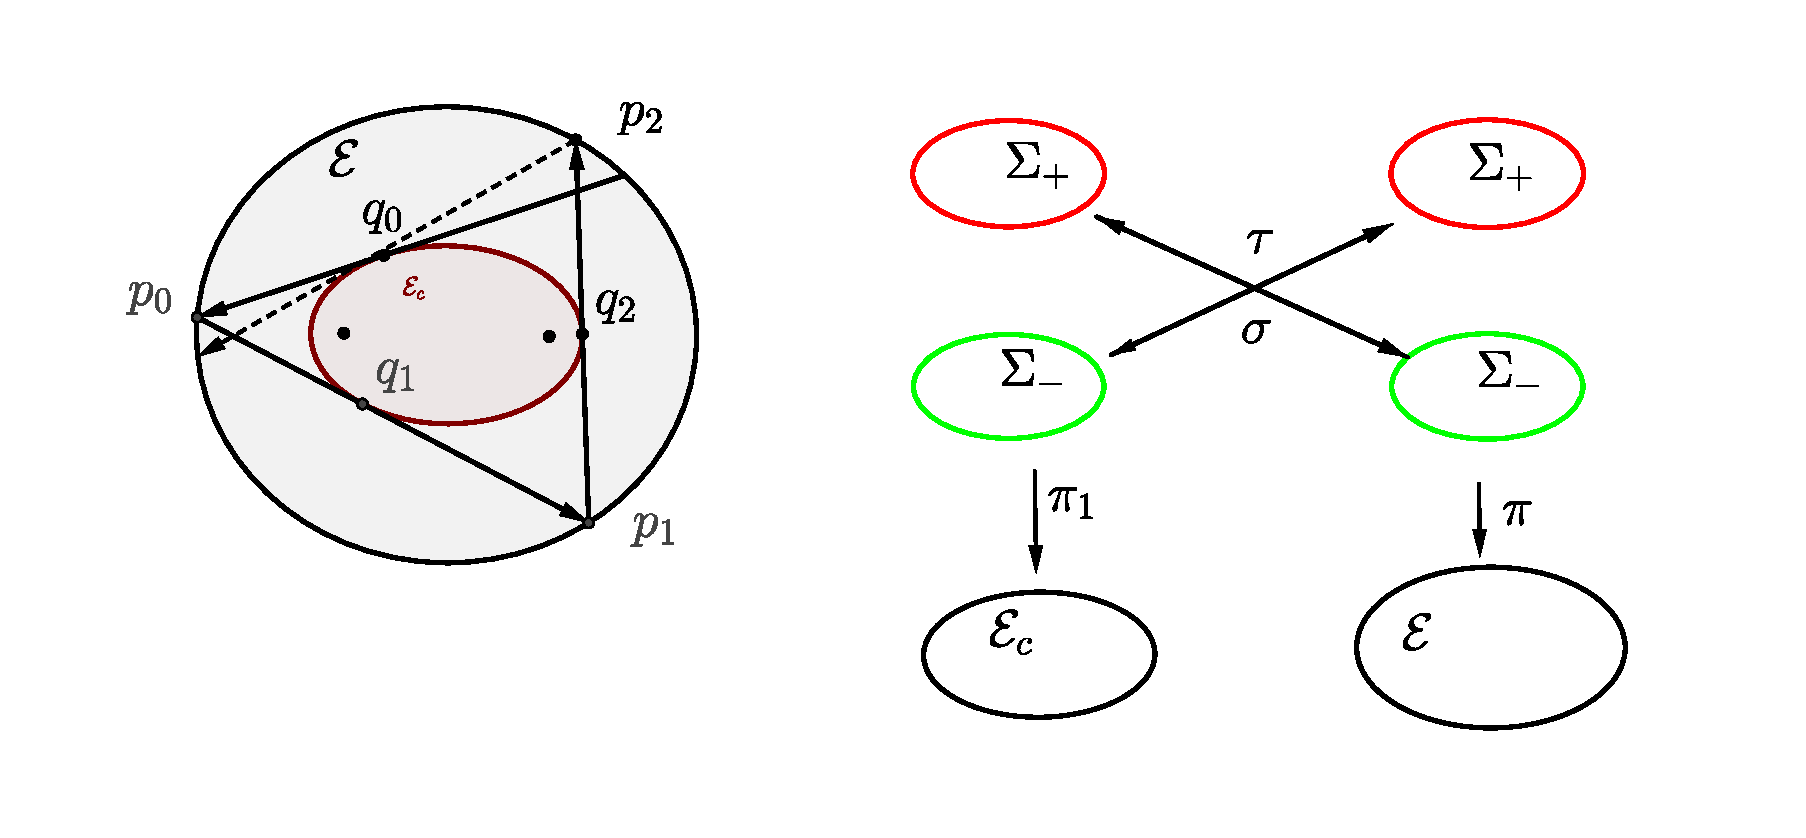
\includegraphics[scale=0.45]{chap_05/pics/pics-05-050-orbitas-dinamica.pdf}
		\caption{Maps $\sigma$, $\tau$ and the the diffeomorphism $\sigma\circ\tau$.}
	\end{center}
\label{fig:caustic2}
\end{figure}


\begin{lemma}
Consider the deck transformations $\sigma$ and $\tau$ as above.
Then
\begin{align*}
   \sigma(x,y,z,w) &=(\bar x, \bar y,z,w),\;\; \tau(x,y,z,w)=(x,y,\bar z,\bar w)\\
   (\bar x,\bar y)&=\left( x - \frac{2 a_c^2        Q_2\, w}{a_c^2  w^2 + b_c^2  z^2}, y + \frac{2  b_c^2     Q_2 z}{a_c^2  w^2 + b_c^2  z^2}\right) \\
   (\bar z,\bar w)&=\left( z+\frac{2a^2 b^2 a_c^4 b_c^2  \,    Q_1\, y}{a^2 b_c^4 x^2 + a_c^4 b^2 y^2}, w-\frac{2 a^2 b^2 a_c^2 b_c^4     Q_1\, x}{a^2 b_c^4 x^2 + a_c^4 b^2 y^2} \right)\\
      Q_1 &=\frac{x w}{ a_c^2 b^2} - \frac{y z}{a^2 b_c^2}, \;\;    Q_2=x w-y z\\
\end{align*}
% antigo sigma nao funciona para Poncelet \left( x-\frac{2 a^4 b^2 a_c^2 b_c^2 %w\,    Q_1}{(a^4 b_c^2 w^2 + a_c^2 b^4 %z^2)} , y+\frac{2 a^2 b^4 z a_c^2 b_c^2 m1}{(a^4 b_c^2 w^2 + a_c^2 b^4 z^2) }\right)
\end{lemma}

\begin{proof} Direct from the definitions of $\sigma$ and $\tau$. The line passing through $(x,y)$ and $(\bar x, \bar y)$ is the polar line of $(z,w)$ with respect to $\mathcal{E}_c$. Also the line passing through $(z,w) $ and $(\bar z,\bar w)$ is tangent to $\mathcal{E}_c$ at $(x,y)$. It is useful to write $\sigma=\sigma_{\pm}$ and $\tau=\tau_{\pm}$. See \cref{fig:05-pics-poncelet-bryant}.
\begin{figure}
    \centering
    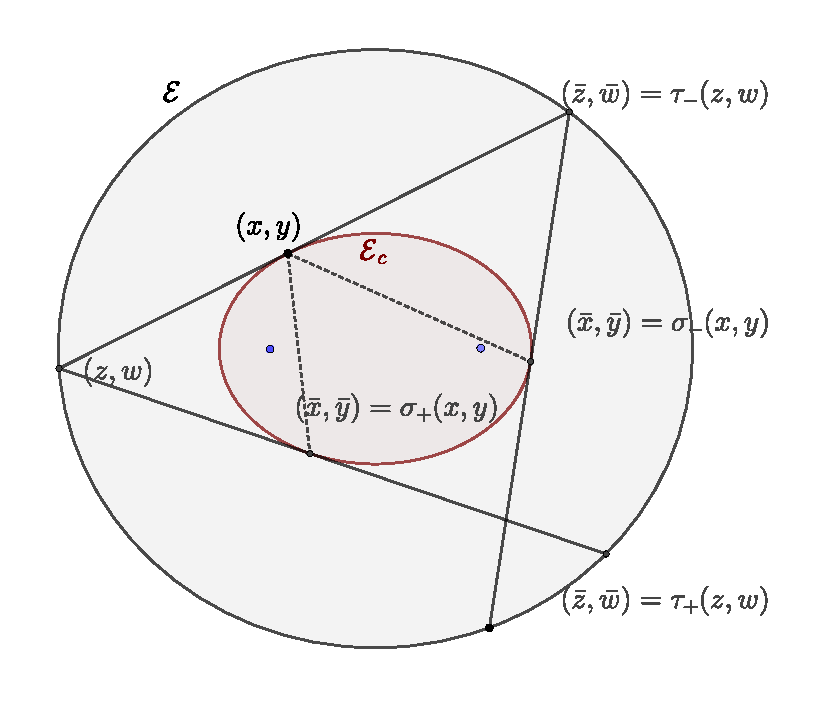
\includegraphics[scale=0.5]{chap_05/pics/pics-05-0010-bryant_poncelet_pair.pdf}
    \caption{Deck transformations $\sigma (x,y,z,w)=(\bar x,\bar y,z,w)=(\sigma_{\pm}(x,y),z,w)$ and $\tau_{\pm}(x,y,z,w)=(x,y,\bar z,\bar w)= (x,y, \tau_{\pm}(z,w) )$. }
    \label{fig:05-pics-poncelet-bryant}
\end{figure}
\end{proof}

\begin{lemma} Let $p=(x,y,z,w)$.
Then:
\[
       Q_2(p)+   Q_2(\sigma(p))=0,\;\;     Q_1(p)+   Q_1(\tau(p))=0
\]
\label{lem:05-m-odd}
\end{lemma}

\begin{proof} Straightforward calculations.
\end{proof}

\begin{proposition}
Then expressions below define a differential 1-form in $\Sigma.$

\begin{align*}
  d\theta=  -\frac{dx}{ a_c^2 y\,    Q_1}& =  \frac{dy}{b_c^2 x\,    Q_1}= -\frac{b^2dz}{w\,    Q_2}=\frac{a^2 dw}{z \,   Q_2}\\
 %      Q_1&=\frac{x w}{ a_c^2 b^2} - \frac{y z}{a^2 b_c^2} , \;\;   Q_2=x w-y z
\end{align*}
\end{proposition}

\begin{proof}
The expressions stated are obtained solving the system of equations $df=dg=dh=0$. Since $\Sigma$ is a regular curve, it follows that each expression is non null in open arcs and by the Implicit Function Theorem   they cannot be zero simultaneously. Therefore, $d\theta$ is a well defined 1-form.
\end{proof}
\begin{remark}
\[ d\theta=\frac{(  b^2   z dw  - a^2  w dz     )   a^2   b^2}{    Q_2   (a^4   w^2 + b^4   z^2)}=\frac{(b_c^2  x dy -a_c^2  y dx         )}{   Q_1   (a_c^4   y^2 + b_c^4   x^2)}
\]
\end{remark}
\begin{proposition}
\[ \sigma^{*}(d\theta)=-d\theta,\;\; \tau^{*}(d\theta)=-d\theta \]
\label{prop:05-invariant-measure}
\end{proposition}

\begin{proof} Follows from \cref{lem:05-m-odd}.
\end{proof}

Now consider a positive  orientation in $\Sigma_+$ such $d\theta$ is a positive 1-form, and define
\[ L=\int_{\Sigma_+ } d\theta >0\]

Define the map
$\theta:\Sigma_+\to \mathbb{R}/(L \mathbb{Z})$ by

\[\theta(x,y,z,w)=\left(\int_{p_0}^p d\theta\right) \text{mod} L ,\;\; p_0=(1,0,z_0,w_0),\; p=(x,y,z,w)\]

\begin{theorem}
The map $\theta $ is a conjugation of $\tau\circ \sigma$ and a translation $T:\mathbb{R}/(L\mathbb{Z})\to \mathbb{R}/(L\mathbb{Z})$ given by $T(x)=x+\alpha$, for some $\alpha$.
\label{thm:05-rotation-cirle}
\end{theorem}

\begin{proof}
By \cref{prop:05-invariant-measure} it follows that $(\tau\circ \sigma)^{*}(d\theta)=d\theta$, i.e., it preserves a regular measure $d\theta$ on $\Sigma_+$ that is diffeomorphic to a circle. 

 
\begin{tikzpicture}
  \matrix (m) [matrix of math nodes,row sep=3em,column sep=4em,minimum width=2em]
  {  \Sigma_+ & \Sigma_+\\
     \mathbb{R}/(L\mathbb{Z}) & \mathbb{R}/(L\mathbb{Z}) \\};
  \path[-stealth]
    (m-1-1) edge node [left] {$\theta $} (m-2-1)
            edge  node [above] {$\tau\circ\sigma  $} (m-1-2)
    (m-2-1.east|-m-2-2) edge node [above] {$T_\alpha$}
            node [above] { } (m-2-2)
    (m-1-2) edge node [right] {$\theta$} (m-2-2);
      %     edge [dashed,-] (m-2-1);
\end{tikzpicture}

Therefore, $\tau\circ\sigma$ is conjugated to a rotation of the circle.
\end{proof}

\begin{remark} The number $\alpha/L$ is the rotation number of the diffeomorphism $f=\tau\circ\sigma$.   Considering an orbit $p_0, p_1, p_2,\ldots, $ it follows that
\[ \rho(f)=\frac{\alpha}{L}=\lim_{n\infty}\left(\frac{1}{n} \sum_{i=0}^{n}\int_{p_i}^{p_{i+1}} F(p)d\theta \right) \]

See \cite{franks-2003}. 

 

\textcolor{red}{corrigir usando teorema de Franks para definir F(p) no nosso caso}
In our discussion, 
  the rotation number is a measure of a segment of an orbit over the total measure of $\Sigma$. 
 For example, we can compute:
\begin{align*}
  \alpha &= \int_{p_0}^{p_{1}}d\theta&= \int_{x_1}^ {a_c}\frac{dx}{a_c^2y Q_1} \\ p_0&=\left[1,0,a_c,-\frac{b\sqrt{a^2 - ac^2}}{a}\right], \;p_1=\left[x_1,y_1, a_c,\frac{b\sqrt{a^2 - ac^2}}{a}\right]\\
    x_1&=-\frac {a_c\, \left( {a}^{2}({b}^{2}- b_c^{2})-{b}^{2}a_c^{2} \right) }{a^{2}(b^{2}+ b_c^{2})-b^{2}
a_c^2}, \; y_1= \,\frac {2 a b_c^{2}b\sqrt {{a}^{2}-a_c^{2}}}{ \left( {b}^{2}+b_c^{2} \right) {a}^{2}-{b}^{2}a_c^2}
    \end{align*}
 
\end{remark}
In  \cite{kolod1985} the rotation number of an elliptic billiard  is explicitly derived and expressed in terms of elliptic functions.
\textcolor{red}{checar notacao abaixo}
\begin{theorem}
  \label{th:cap5-rotation-number} Let $T$ be the billiard map such that all orbits are simple. Then
the rotation number of $T$ is equal to
\begin{equation}
    \frac{1}{2}- \frac{F(\beta/2,k)}{F(\pi/2,k}
\end{equation}
where $F(\alpha,k)$ is the elliptic integral
\[ F(\alpha,k)=\int_0^{\alpha} \frac{dx}{\sqrt{1-k^2 \sin^2x}}\]
and
\begin{align*}
\alpha&=\frac{1}{4c^2}\frac{f^2-e^2}{(1-f^2)(1-e^2)},\; e=a/c, f=a_c/c\\
\beta&=\frac{1-f^2 }{1-e^2}\arcsin{\frac{e}{f}},\;\;\; k=\frac{2+\sqrt{2}}{1+f}.    
\end{align*}
\end{theorem}
 
\begin{corollary} 
In   above conditions  the Poncelet pair $\{\E,\E_c\}$ has a $N-$periodic orbit if and only if $\alpha/L$ is rational.
\end{corollary}

 
\begin{proof} Direct from \cref{thm:05-rotation-cirle}.
\end{proof}
%\begin{remark} Most of this section was based in \cite{bry-2010}.
%\end{remark}